\section{Introduction}


%%%%%%%%%%%%%%%%%%%%%%%%%%%%%%%%%%%%%%%%%%%%%%%%%%%%%%%%%%%%%%%%%%%%%%%%%%%%%%%
\section{Methodology}

Starting with \citet{Thompson1982} and \citet{Reid1990}, Euler's equation has
been used to estimate the source positions of gravity and magnetic data.
In this section, we will review the solution of Euler's equation for
$(x_o, y_o, z_o)$ by Euler deconvolution \citep{Reid1990} and then present a
new method, called \textit{Euler inversion}, for solving Euler's equation using
total least-squares.

We start with Euler's homogeneity equation

\begin{equation}
  (x - x_o)\partial_x f + (y - y_o)\partial_y f + (z - z_o)\partial_z f
  + \eta(f - b) = 0
  \ ,
  \label{eq:euler}
\end{equation}

\noindent
in which $f$ is a homogeneous function (in this case, a potential-field),
$(x, y, z)$ are the coordinates of the observation point,
$(x_o, y_o, z_o)$ are the coordinates of the field source,
$b$ is the base level representing a constant shift in the field,
and $\eta$ is the structural index, which is related to the nature of the
source and how its potential-field values decay with distance \citep{Reid2014}.
Equation~\ref{eq:euler} relates the coordinates of the source with the observed
potential field and its gradient.

Given $N$ observations points in which we have measured $f$ and its gradient
(for a total $4N$ data), both Euler deconvolution and Euler inversion aim to
estimate the parameter vector

\begin{equation}
  \mathbf{p} = \begin{bmatrix}x_o & y_o & z_o & b \end{bmatrix}^T.
  \label{eq:p}
\end{equation}

\subsection{Euler deconvolution}

Euler deconvolution starts by rearranging Equation~\ref{eq:euler} to place the
parameters on the left-hand side and all other terms on the right-hand side.
This is an attempt to form a \textit{parametric model} which results in the
$N \times 4$ equation system

\begin{equation}
  \begin{aligned}
  -x_o\partial_x f_1 - y_o\partial_y f_1 - z_o\partial_z f_1 - \eta b &= -x_1\partial_x f_1 - y_1\partial_y f_1 - z_1\partial_z f_1 - \eta f_1
  \\
  -x_o\partial_x f_2 - y_o\partial_y f_2 - z_o\partial_z f_2 - \eta b &= -x_2\partial_x f_2 - y_2\partial_y f_2 - z_2\partial_z f_2 - \eta f_2
  \\
  \vdots
  \\
  -x_o\partial_x f_N - y_o\partial_y f_N - z_o\partial_z f_N - \eta b &= -x_N\partial_x f_N - y_N\partial_y f_N - z_N\partial_z f_N - \eta f_N
  \end{aligned}
  \ ,
\end{equation}

\noindent
which can be written in matrix form as

\begin{equation}
  \underbrace{
    \begin{bmatrix}
      -\partial_x f_1 & -\partial_y f_1 & -\partial_z f_1 & -\eta \\
      -\partial_x f_2 & -\partial_y f_2 & -\partial_z f_2 & -\eta \\
      \vdots & \vdots & \vdots & \vdots \\
      -\partial_x f_N & -\partial_y f_N & -\partial_z f_N & -\eta
    \end{bmatrix}
  }_{\mathbf{A}}
  \underbrace{
    \begin{bmatrix}
      x_o \\ y_o \\ z_o \\ b
    \end{bmatrix}
  }_{\mathbf{p}}
  =
  \underbrace{
    \begin{bmatrix}
      -x_1\partial_x f_1 - y_1\partial_y f_1 - z_1\partial_z f_1 - \eta f_1 \\
      -x_2\partial_x f_2 - y_2\partial_y f_2 - z_2\partial_z f_2 - \eta f_2 \\
      \vdots \\
      -x_N\partial_x f_N - y_N\partial_y f_N - z_N\partial_z f_N - \eta f_N \\
    \end{bmatrix}
  }_{\mathbf{c}}
  \ ,
  \label{eq:deconv-system}
\end{equation}

\noindent
in which $\mathbf{A}$ is the Jacobian matrix of Euler's equation
(Equation~\ref{eq:euler}) with respect to the parameters
(Equations~\ref{eq:p})
and $\mathbf{c}$ is a \textit{pseudo-data vector}.

The solution proposed by \citet{Thompson1982} and \citet{Reid1990} is a
least-squares estimate of $\mathbf{p}$

\begin{equation}
  \hat{\mathbf{p}} = \left(\mathbf{A}^T\mathbf{A}\right)^{-1}
  \mathbf{A}^T\mathbf{c}
  \ .
  \label{eq:deconv-p}
\end{equation}

\noindent
However, the solution above is valid only if the contents of the Jacobian
matrix $\mathbf{A}$ are assumed to be error-free.
As can be seen from Equation~\ref{eq:deconv-system}, the Jacobian contains the
derivatives of $f$, which are often computed numerically by finite-differences
or Fourier transforms and are known to amplify the high-frequency random noise
in the data.
This presents a problem, particularly for the estimation of $z_o$, which has
been widely explored in the literature [CITATION NEEDED].


\subsection{Euler inversion}

Euler inversion starts by assigning a $4N \times 1$ \textit{data vector}
which contains all of the observations of $f$ and its gradient

\begin{equation}
  \mathbf{d} =
  \begin{bmatrix}
    f_1 & \cdots & f_N &
    \partial_x f_1 & \cdots & \partial_x f_N &
    \partial_y f_1 & \cdots & \partial_y f_N &
    \partial_z f_1 & \cdots & \partial_z f_N
  \end{bmatrix}^T.
  \label{eq:d}
\end{equation}

\noindent
We can the formulate the $N \times 4$ equation system from Euler's equation as
a non-linear function of parameters and data

\begin{equation}
  \mathbf{e}(\mathbf{p}, \mathbf{d}) = \mathbf{0}
  \ ,
  \label{eq:e}
\end{equation}

\noindent
which is known in geodesy as an \textit{implicit model} [CITATION NEEDED].

We then wish to solve the following constrained optimization problem with
non-linear equality constraints to estimate both the parameters and the
predicted data simultaneously

\begin{equation}
  \begin{aligned}
    \min_{\mathbf{p}, \mathbf{d}} \quad &
      \phi(\mathbf{d}) =
      \left[\mathbf{d}^o - \mathbf{d}\right]^T \mathbf{W}
      \left[\mathbf{d}^o - \mathbf{d}\right]
    \\
    \textrm{subject to} \quad &
      \mathbf{e}(\mathbf{p}, \mathbf{d}) = \mathbf{0}
    \ ,
  \end{aligned}
  \label{eq:constrained}
\end{equation}

\noindent
in which $\mathbf{d}^o$ is the \textit{observed data vector} which contains all
of the $4N$ observations of $f$ and its gradient,
$\mathbf{d}$ is the \textit{predicted data vector} from Equation~\ref{eq:d},
and $\mathbf{W}$ is a $4N \times 4N$ diagonal weight matrix.

The constrained problem in Equation~\ref{eq:constrained} can be transformed
into an unconstrained problem by using the Lagrangian

\begin{equation}
  \Lagr(\mathbf{p}, \mathbf{d}, \mathbf{\lambda}) =
    \left[\mathbf{d}^o - \mathbf{d}\right]^T \mathbf{W}
    \left[\mathbf{d}^o - \mathbf{d}\right]
    +
    2 \mathbf{\lambda}^T \mathbf{e}
  \ ,
  \label{eq:lagrangian}
\end{equation}

\noindent
in which $\mathbf{\lambda}$ is an $N \times 1$ vector of Lagrange multipliers.

The non-linear Lagrangian can be minimized through Newton's method by starting
with initial estimates $\mathbf{p}_0$ and $\mathbf{d}_0$ and then iterating
with the corrections to these values through the solution of the linear system

\begin{equation}
  \underbrace{
    \begin{bmatrix}
      \mathbf{H}^{dd}_k & \mathbf{H}^{d\lambda}_k & \mathbf{H}^{dp}_k \\
      \mathbf{H}^{\lambda d}_k & \mathbf{H}^{\lambda\lambda}_k & \mathbf{H}^{\lambda p}_k \\
      \mathbf{H}^{pd}_k & \mathbf{H}^{p\lambda}_k & \mathbf{H}^{pp}_k
    \end{bmatrix}
  }_{\text{Hessian of }\Lagr}
  \begin{bmatrix}
    \mathbf{\Delta d}_k \\
    \mathbf{\Delta \lambda}_k \\
    \mathbf{\Delta p}_k
  \end{bmatrix}
  = -
  \underbrace{
    \begin{bmatrix}
      \mathbf{\nabla}_d\Lagr(\mathbf{p}_k,\mathbf{d}_k,\mathbf{\lambda}_k) \\
      \mathbf{\nabla}_\lambda\Lagr(\mathbf{p}_k,\mathbf{d}_k,\mathbf{\lambda}_k) \\
      \mathbf{\nabla}_p\Lagr(\mathbf{p}_k,\mathbf{d}_k,\mathbf{\lambda}_k)
    \end{bmatrix}
  }_{\substack{\text{gradient}\\ \text{of }\Lagr}}
  \ ,
\end{equation}

\noindent
in which $\mathbf{\nabla}_\alpha$ is the gradient operator with respect to
variable $\alpha$ and
$\mathbf{H}^{\alpha\beta}$ is the Hessian matrix of $\Lagr$ with respect to
variables $\alpha$ and $\beta$.
Since the order of derivation can be swapped in the Hessian matrices, the above
equation can be simplified to

\begin{equation}
    \begin{bmatrix}
      \mathbf{H}^{dd}_k & \mathbf{H}^{d\lambda}_k & \mathbf{H}^{dp}_k \\
      {\mathbf{H}^{d\lambda}_k}^T & \mathbf{H}^{\lambda\lambda}_k & \mathbf{H}^{\lambda p}_k \\
      {\mathbf{H}^{dp}_k}^T & {\mathbf{H}^{\lambda p}_k}^T & \mathbf{H}^{pp}_k
    \end{bmatrix}
  \begin{bmatrix}
    \mathbf{\Delta d}_k \\
    \mathbf{\Delta \lambda}_k \\
    \mathbf{\Delta p}_k
  \end{bmatrix}
  = -
    \begin{bmatrix}
      \mathbf{\nabla}_d\Lagr(\mathbf{p}_k,\mathbf{d}_k,\mathbf{\lambda}_k) \\
      \mathbf{\nabla}_\lambda\Lagr(\mathbf{p}_k,\mathbf{d}_k,\mathbf{\lambda}_k) \\
      \mathbf{\nabla}_p\Lagr(\mathbf{p}_k,\mathbf{d}_k,\mathbf{\lambda}_k)
    \end{bmatrix}
  \ .
  \label{eq:newton}
\end{equation}

Now, we must derive the three gradient vectors and six Hessian matrices in
Equation~\ref{eq:newton}.
We will start with the gradient vectors.

\begin{equation}
  \begin{aligned}
    \mathbf{\nabla}_d\Lagr(\mathbf{p}_k,\mathbf{d}_k,\mathbf{\lambda}_k) &=
      -2\mathbf{W}\left[\mathbf{d}^o - \mathbf{d}_k\right]
      + 2\mathbf{B}_k^T\mathbf{\lambda}_k
    \ ,
    \\
    \mathbf{\nabla}_\lambda\Lagr(\mathbf{p}_k,\mathbf{d}_k,\mathbf{\lambda}_k) &=
      2\mathbf{e}_k
    \ ,
    \\
    \mathbf{\nabla}_p\Lagr(\mathbf{p}_k,\mathbf{d}_k,\mathbf{\lambda}_k) &=
      2\mathbf{A}_k^T\mathbf{\lambda}_k
    \ ,
  \end{aligned}
\end{equation}

\noindent
in which $\mathbf{e}_k = \mathbf{e}(\mathbf{p}_k,\mathbf{d}_k)$, $\mathbf{A}$
is the $N \times 4$ \textit{parameter Jacobian} matrix of Euler's equation
(Equation~\ref{eq:deconv-system}), and $\mathbf{B}$ is the $N \times 4N$
\textit{data Jacobian} of Euler's equation which is composed of four diagonal
matrices

\begin{equation}
  \begin{gathered}
  \mathbf{B} =
  \begin{bmatrix}
    \mathbf{B}^f &
    \mathbf{B}^x &
    \mathbf{B}^y &
    \mathbf{B}^z
  \end{bmatrix}
  , \quad
  \mathbf{B}^f =
  \begin{bmatrix}
    \eta & \cdots & 0 \\
    \vdots & \ddots & \vdots \\
    0 & \cdots & \eta
  \end{bmatrix}
  ,
  \\
  \mathbf{B}^x =
  \begin{bmatrix}
    x_1 - x_o & \cdots & 0 \\
    \vdots & \ddots & \vdots \\
    0 & \cdots & x_N - x_o
  \end{bmatrix}
  , \quad
  \mathbf{B}^y =
  \begin{bmatrix}
    y_1 - y_o & \cdots & 0 \\
    \vdots & \ddots & \vdots \\
    0 & \cdots & y_N - y_o
  \end{bmatrix}
  , \quad
  \mathbf{B}^z =
  \begin{bmatrix}
    z_1 - z_o & \cdots & 0 \\
    \vdots & \ddots & \vdots \\
    0 & \cdots & z_N - z_o
  \end{bmatrix}
  \end{gathered}
  \ .
\end{equation}


\subsection{Estimating the structural index}

\subsection{Windowing procedure}


%%%%%%%%%%%%%%%%%%%%%%%%%%%%%%%%%%%%%%%%%%%%%%%%%%%%%%%%%%%%%%%%%%%%%%%%%%%%%%%
\section{Results}


\subsection{Method demonstration with a single window}

\begin{figure}[tb!]
\centering
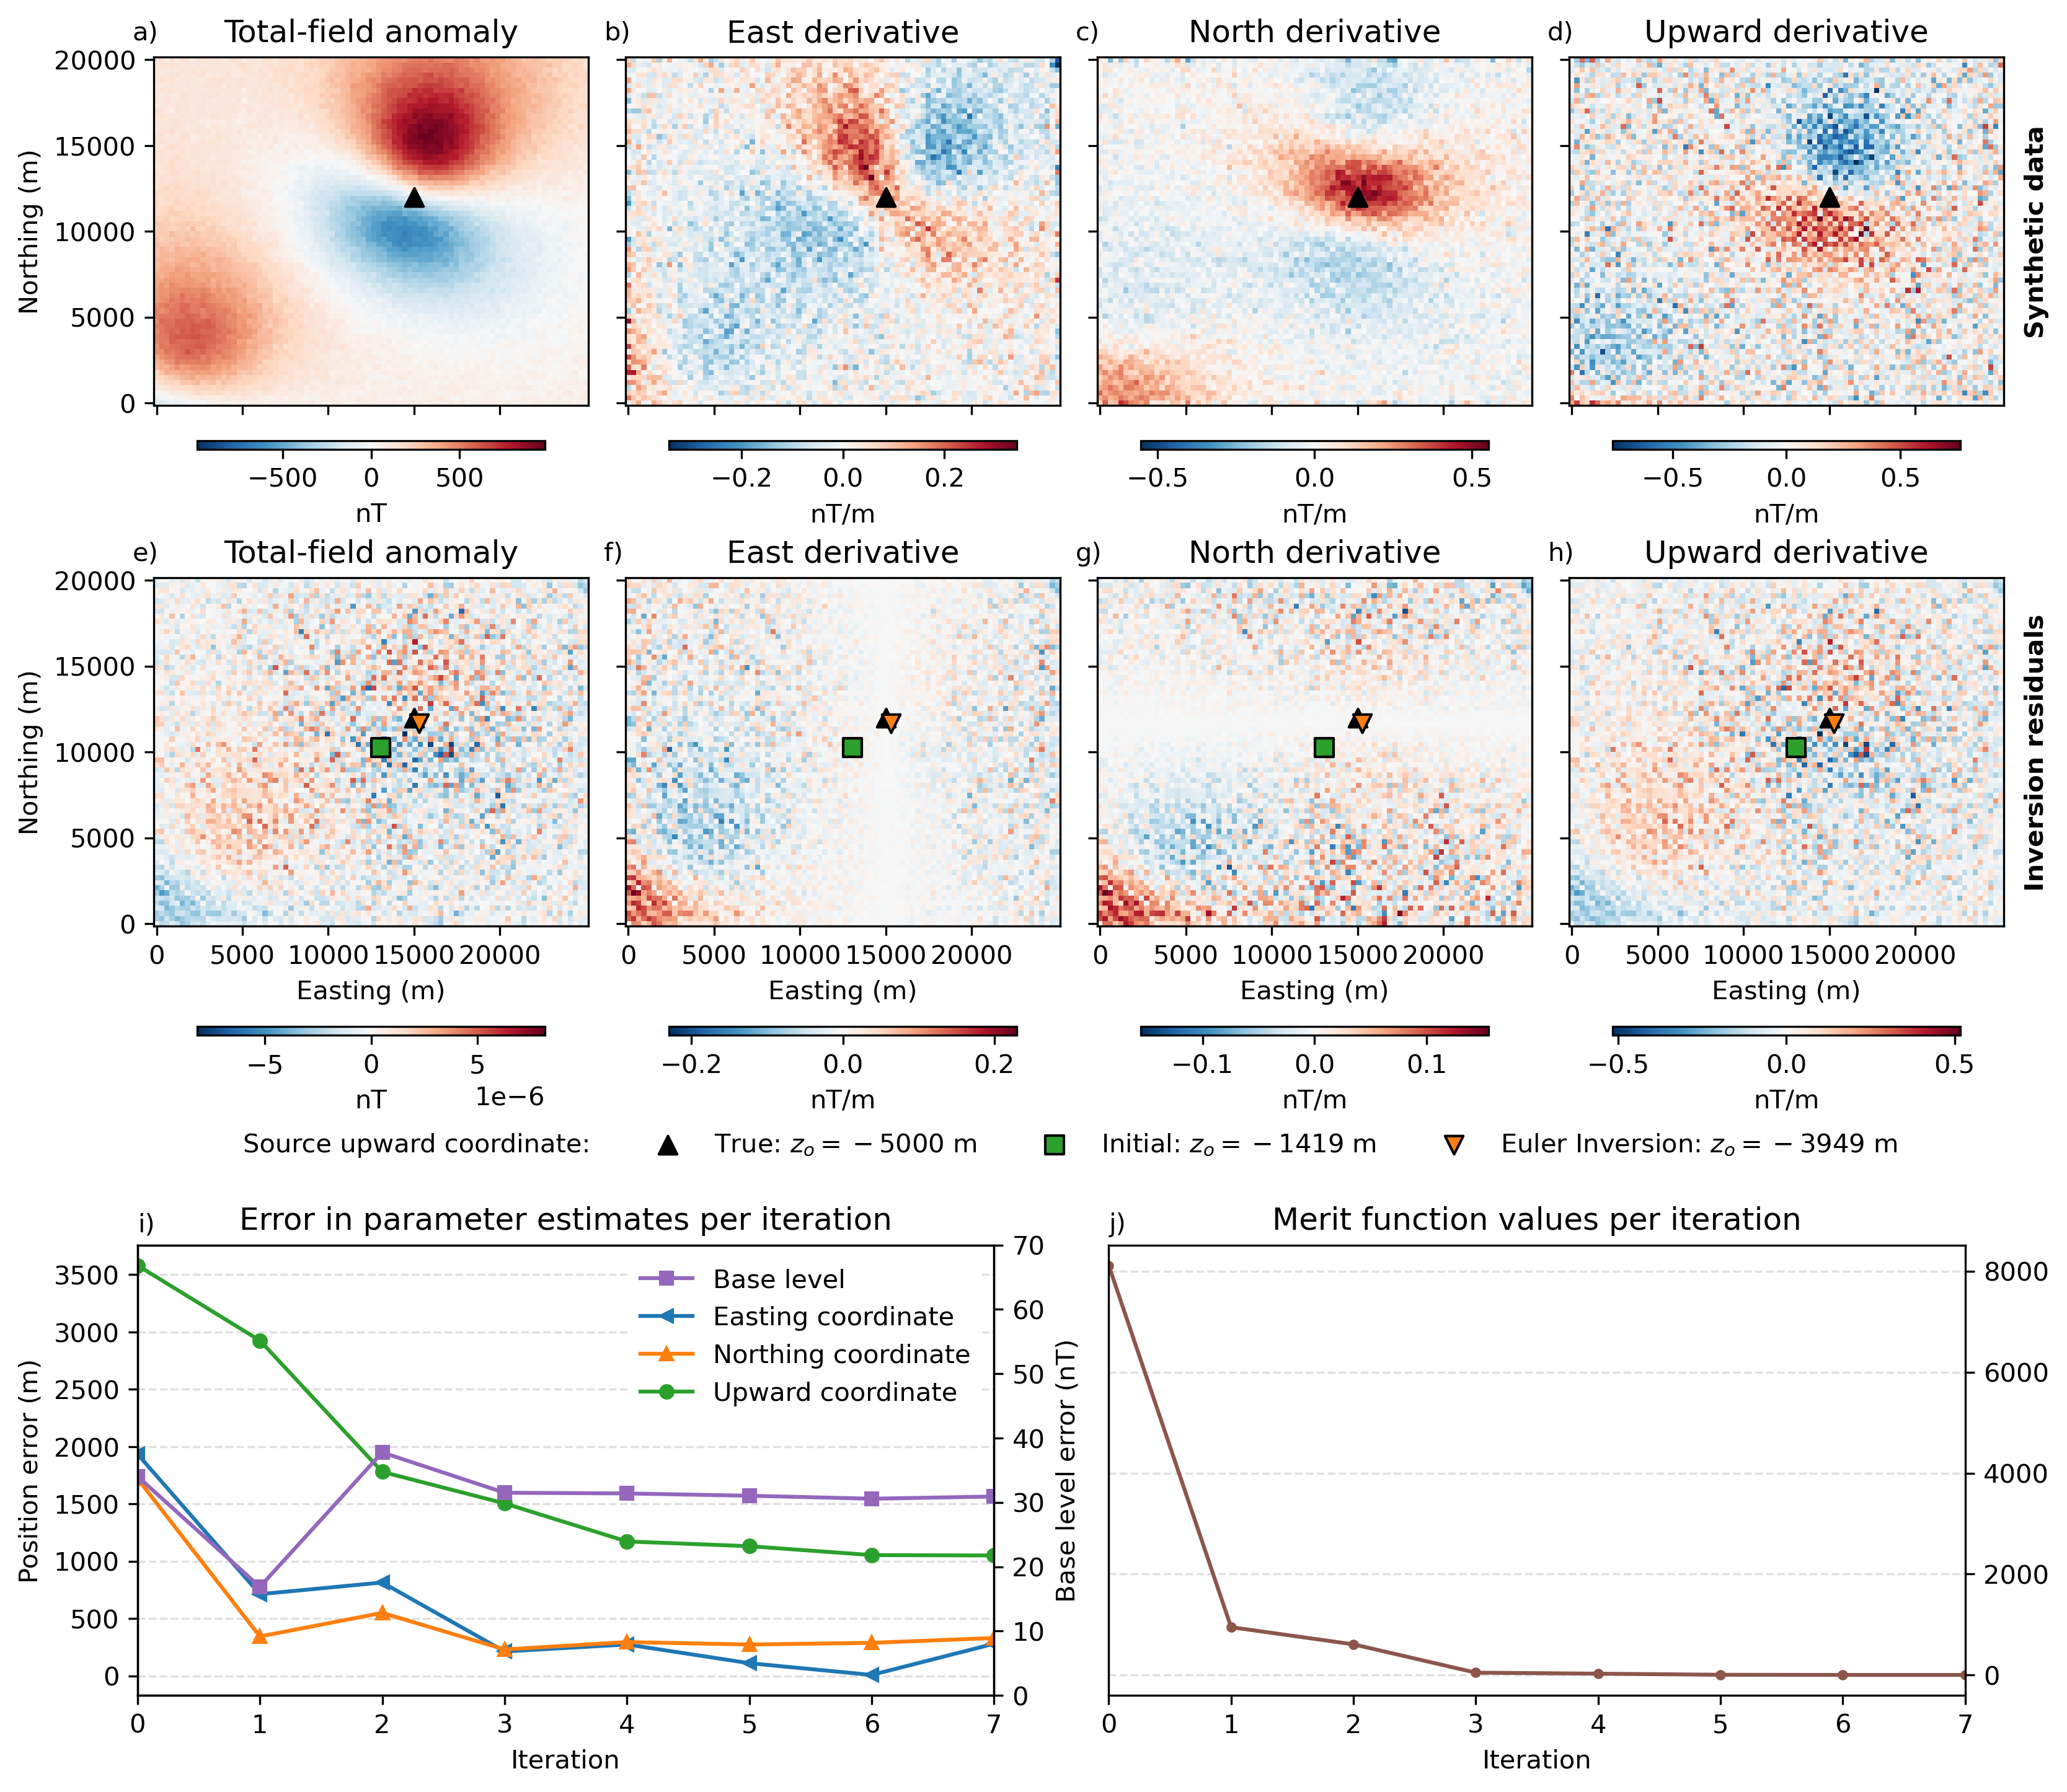
\includegraphics[width=1\linewidth]{figures/synthetic-proof-of-concept.png}
\caption{
  \lipsum[1]
}
\label{fig:proof}
\end{figure}


\subsection{Effect of random noise}

\begin{figure}[tb!]
\centering
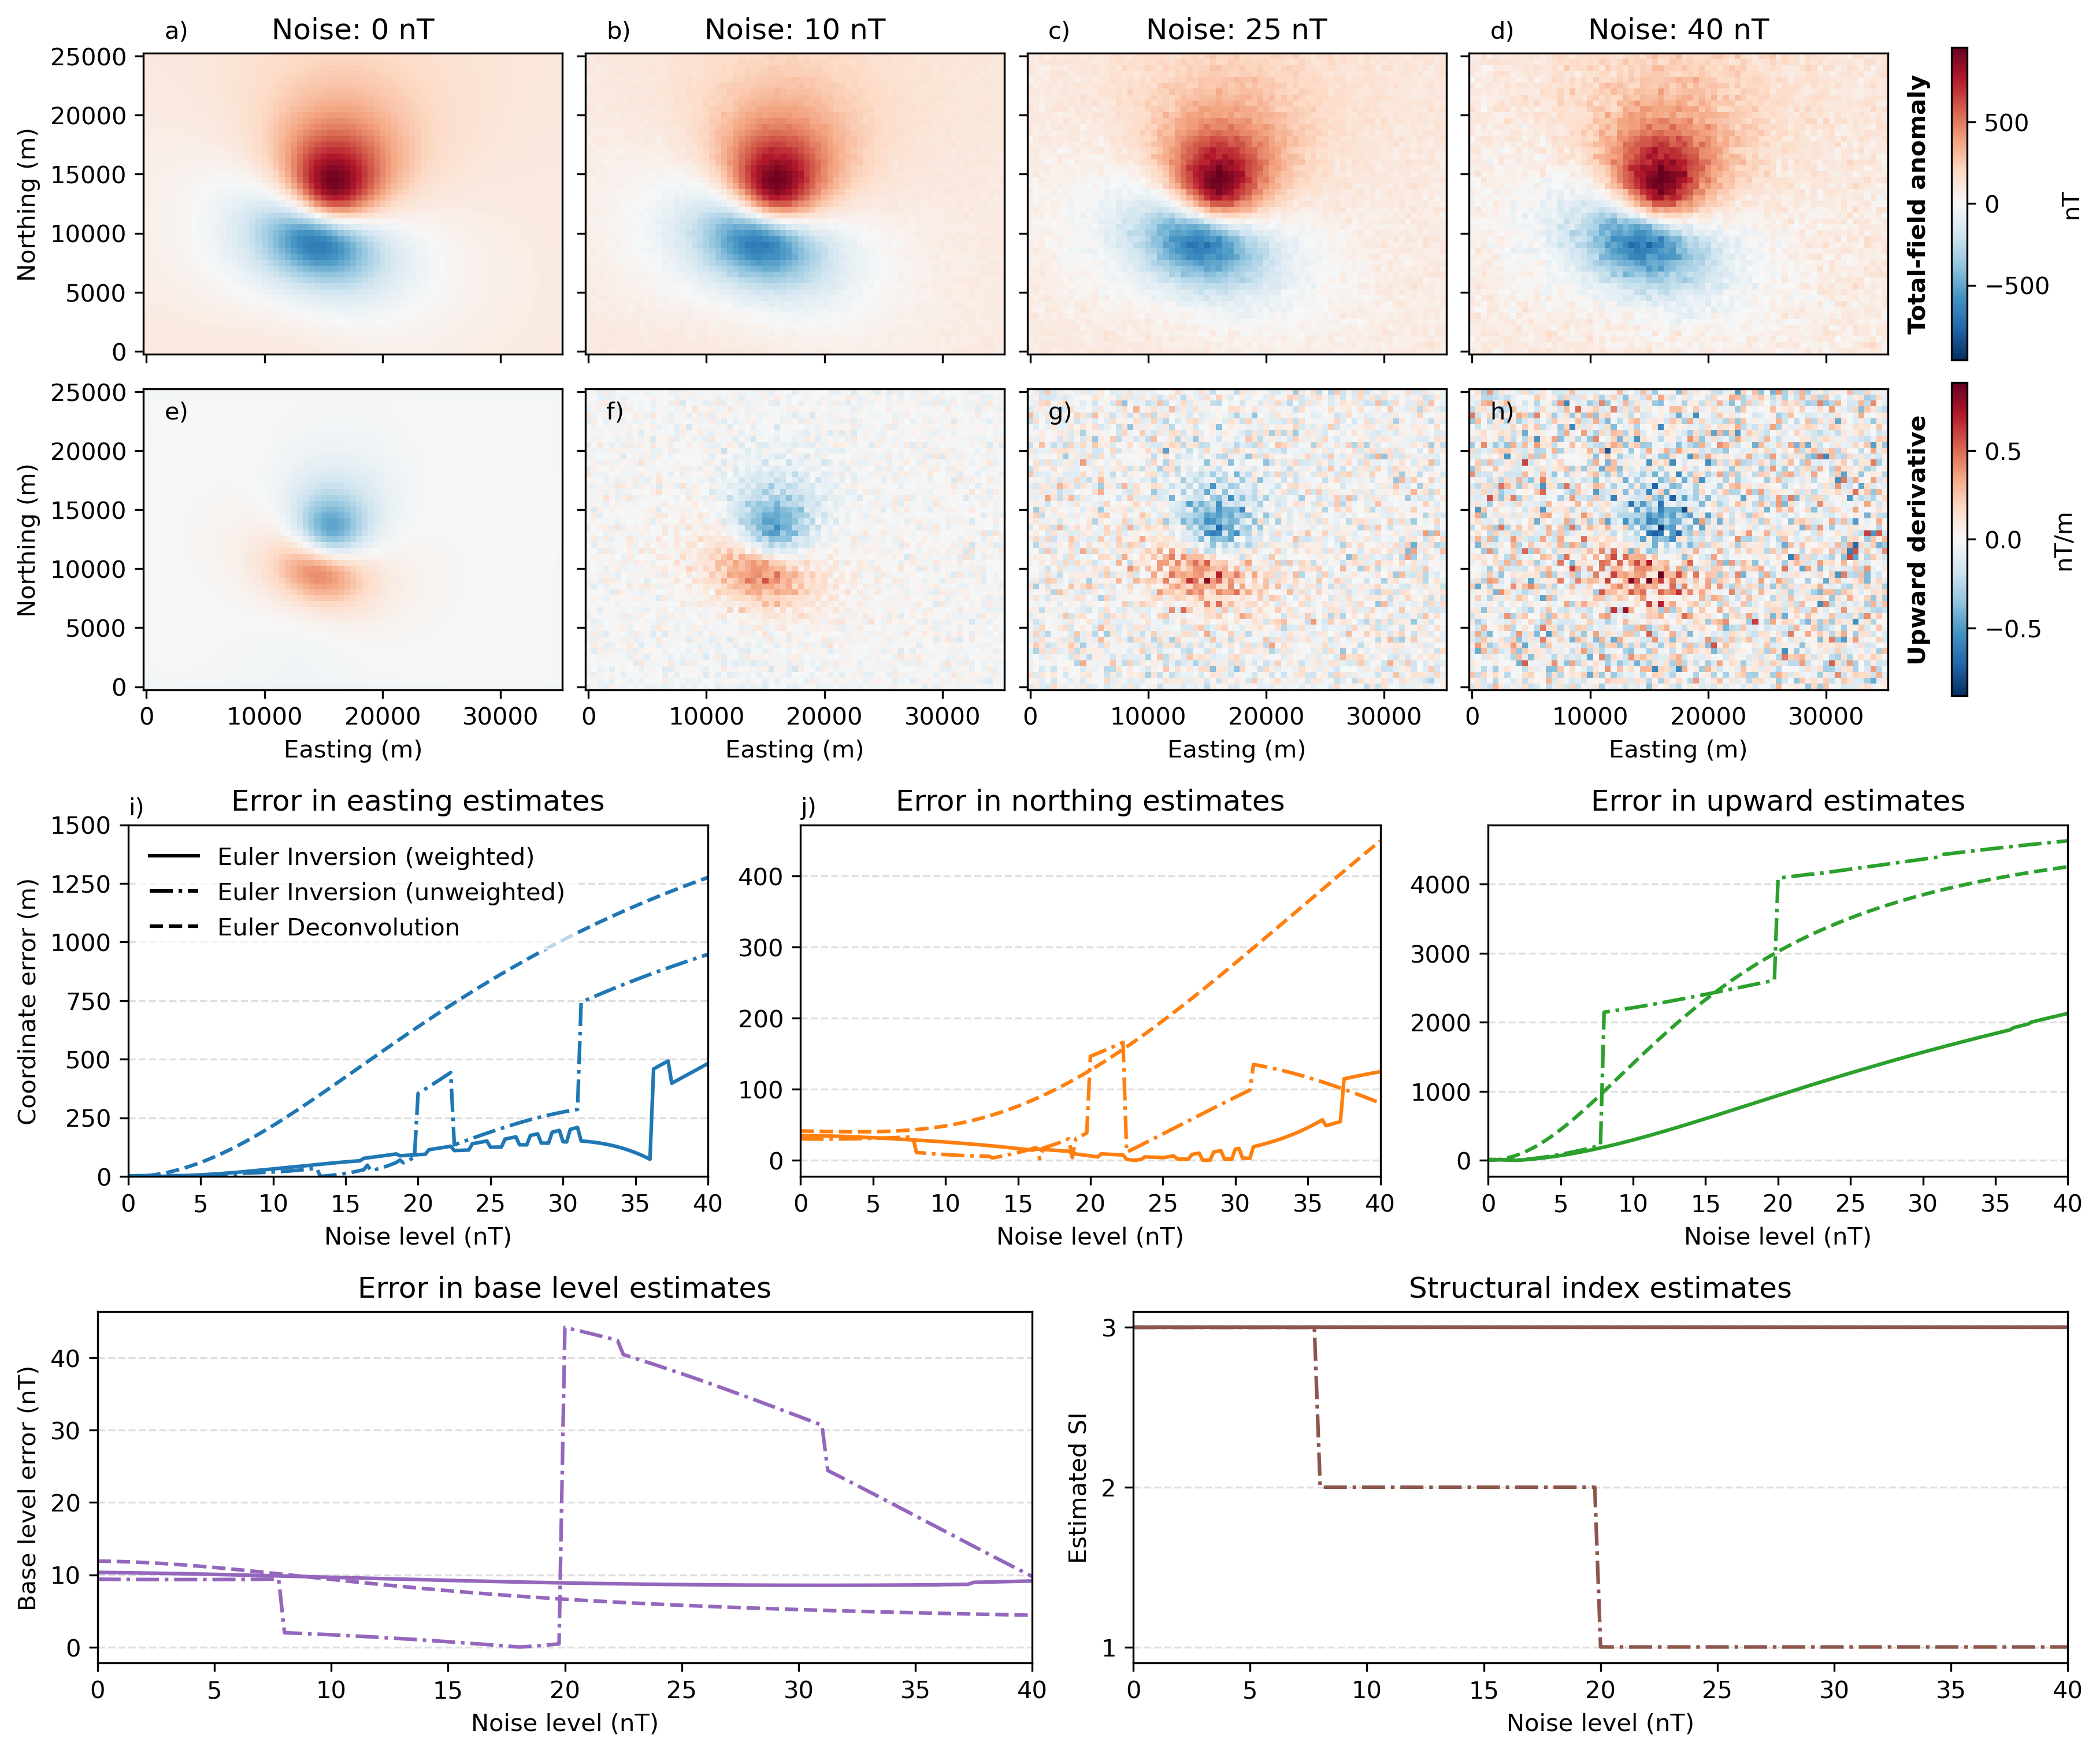
\includegraphics[width=1\linewidth]{figures/synthetic-noise-levels.png}
\caption{
  \lipsum[1]
}
\label{fig:noise}
\end{figure}

\subsection{Effect of SI on multiple sources}

\begin{figure}[tb!]
\centering
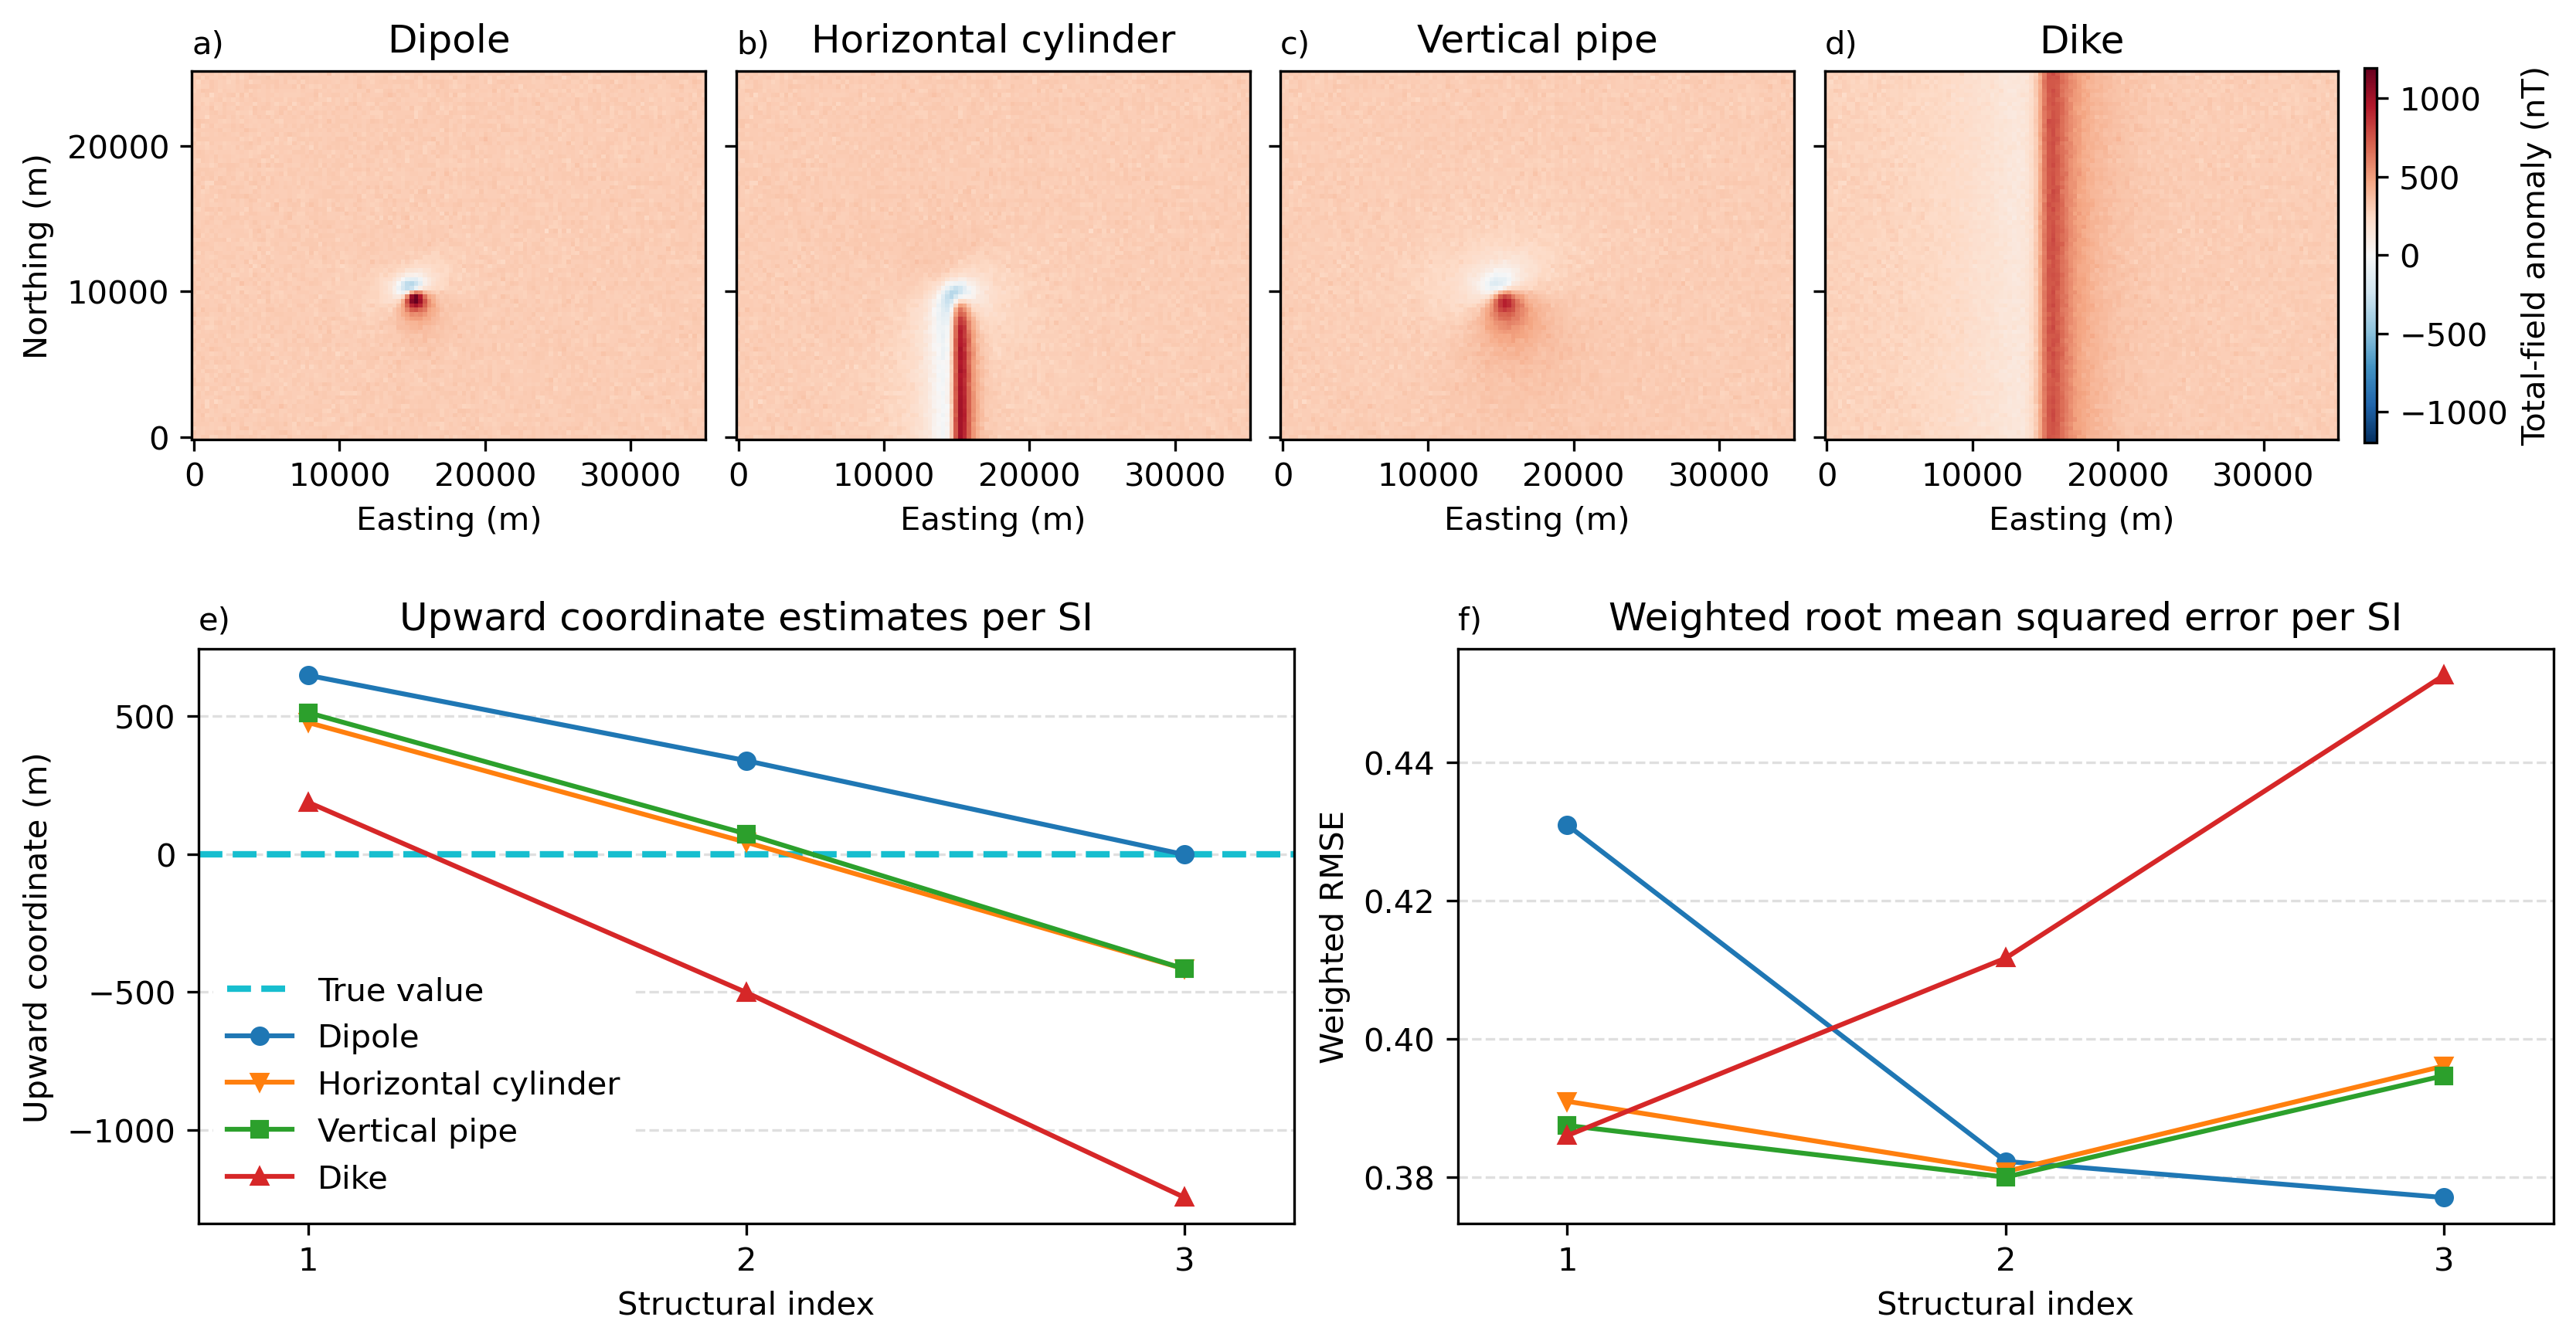
\includegraphics[width=1\linewidth]{figures/synthetic-structural-index.png}
\caption{
  \lipsum[1]
}
\label{fig:si}
\end{figure}

\subsection{Windowing procedure with multiple sources}

\begin{figure}[tb!]
\centering
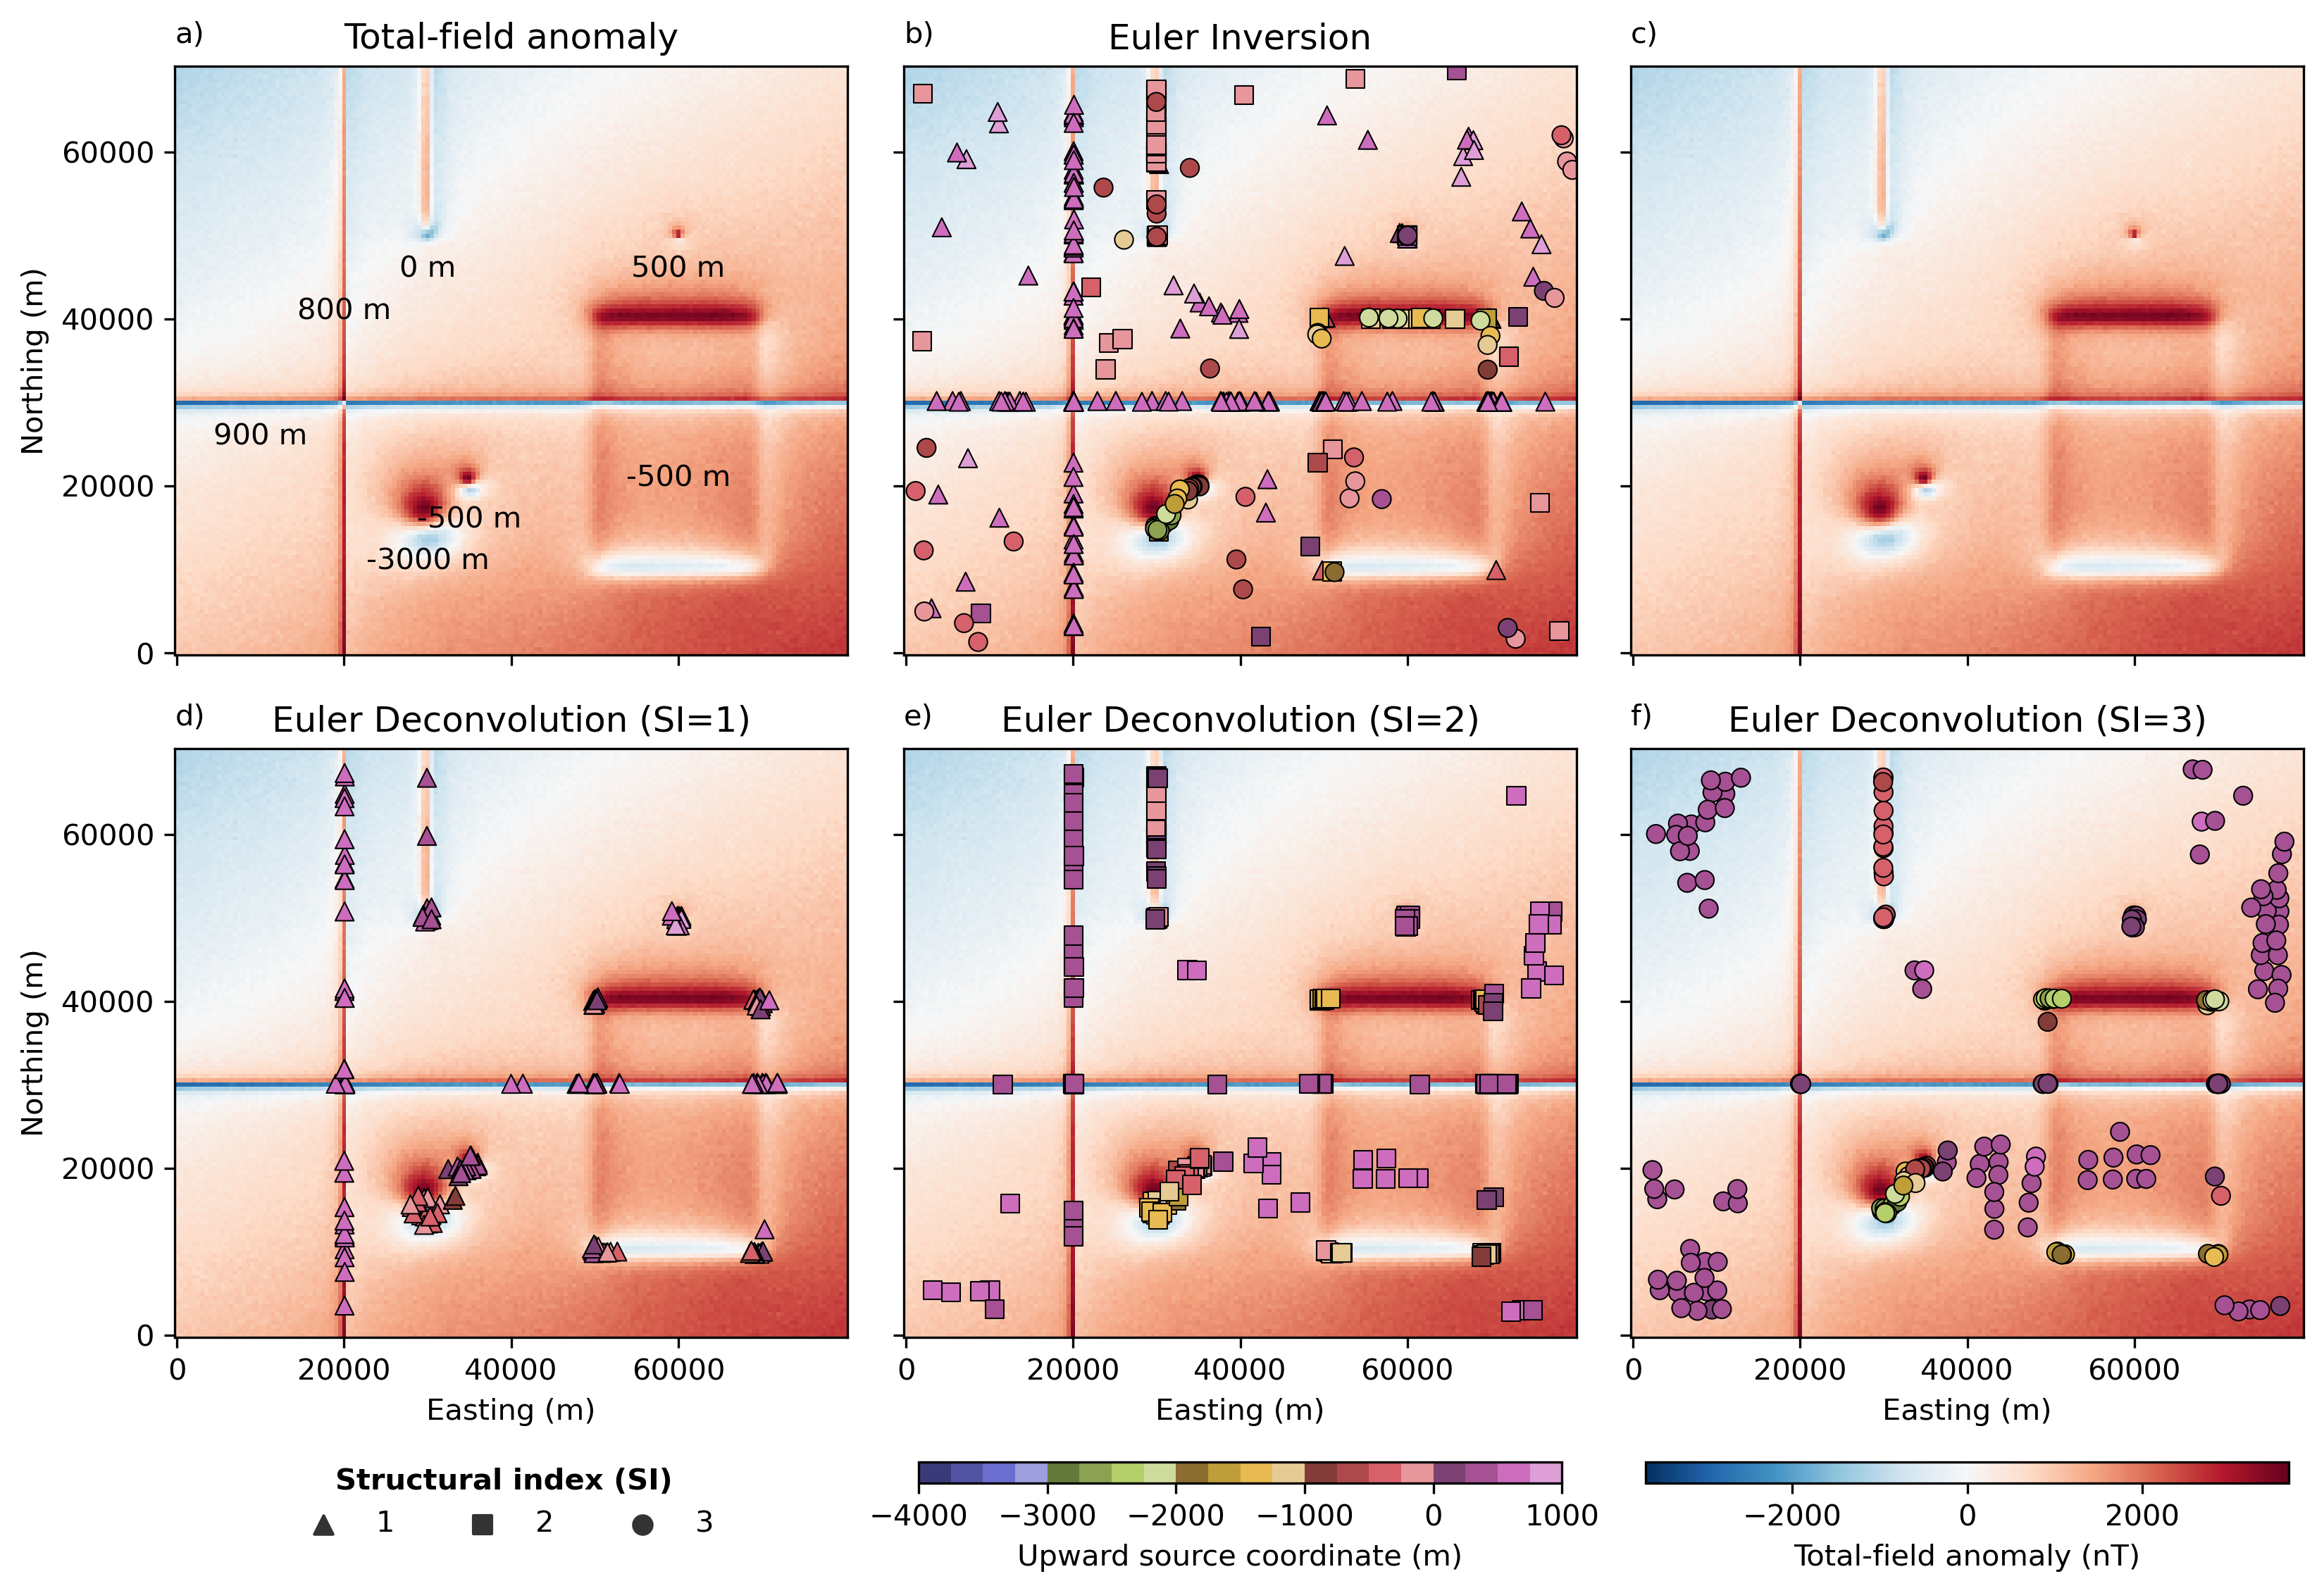
\includegraphics[width=1\linewidth]{figures/synthetic-windows.png}
\caption{
  \lipsum[1]
}
\label{fig:windows}
\end{figure}

\subsection{Aeromagnetic data from Rio de Janeiro}

%%%%%%%%%%%%%%%%%%%%%%%%%%%%%%%%%%%%%%%%%%%%%%%%%%%%%%%%%%%%%%%%%%%%%%%%%%%%%%%
\section{Conclusion}



%%%%%%%%%%%%%%%%%%%%%%%%%%%%%%%%%%%%%%%%%%%%%%%%%%%%%%%%%%%%%%%%%%%%%%%%%%%%%%%
\section{Open research}

The Python source code used to produce all results and figures presented here
is available at \url{https://github.com/\GitHubRepository} and
\url{https://doi.org/\ArchiveDOI} under the MIT open-source license.

Here we should cite all of the main software used, like Jupyter, numpy, scipy,
matplotlib, Fatiando, etc.

Cite any data sources as well.



%%%%%%%%%%%%%%%%%%%%%%%%%%%%%%%%%%%%%%%%%%%%%%%%%%%%%%%%%%%%%%%%%%%%%%%%%%%%%%%
\section{Acknowledgements}

We are indebted to the developers and maintainers of the open-source software
without which this work would not have been possible.
Acknowledge any non-author contributors to this study.
Statement about funding.

% Thank the editors and reviewers after review.
